%% LyX 2.4.2.1 created this file.  For more info, see https://www.lyx.org/.
%% Do not edit unless you really know what you are doing.
\documentclass[12pt,english]{beamer}
\usepackage{mathpazo}
\renewcommand{\familydefault}{\rmdefault}
\usepackage[T1]{fontenc}
% \usepackage[latin9]{inputenc}
\setcounter{secnumdepth}{3}
\setcounter{tocdepth}{3}
\usepackage[active]{srcltx}
\usepackage{amsthm}
\usepackage{amsmath} 
\usepackage{amssymb}
\usepackage[authoryear]{natbib}
\usepackage{graphicx}
\usepackage[UTF8]{ctex} % Enable Chinese support

\makeatletter
%%%%%%%%%%%%%%%%%%%%%%%%%%%%%% Textclass specific LaTeX commands.
% this default might be overridden by plain title style
\newcommand\makebeamertitle{\frame{\maketitle}}%
% (ERT) argument for the TOC
\AtBeginDocument{%
  \let\origtableofcontents=\tableofcontents
  \def\tableofcontents{\@ifnextchar[{\origtableofcontents}{\gobbletableofcontents}}
  \def\gobbletableofcontents#1{\origtableofcontents}
}
\theoremstyle{definition}
\newtheorem*{example*}{\protect\examplename}
\theoremstyle{definition}
\newtheorem*{defn*}{\protect\definitionname}
\theoremstyle{plain}
\newtheorem*{thm*}{\protect\theoremname}

%%%%%%%%%%%%%%%%%%%%%%%%%%%%%% User specified LaTeX commands.
\AtBeginDocument{%
   \let\origtableofcontents=\tableofcontents
   \def\tableofcontents{\@ifnextchar[{\origtableofcontents}{\gobbletableofcontents}}
   \def\gobbletableofcontents#1{\origtableofcontents}
 }\usepackage[english]{babel}
\usepackage{babel}

%\usetheme{Boadilla}
\usetheme{Madrid}
\setbeamertemplate{navigation symbols}{}
% \usecolortheme{orchid}
\usecolortheme{spruce}
% \usecolortheme{beaver}

\setbeamercovered{transparent}

\usepackage{colortbl}

\usefonttheme[onlymath]{serif}
%%%%%%%%%%%%%%%%%%%%%%%%

% For tables
\usepackage{multirow}
\usepackage{array}
\usepackage{rotating}
\usepackage{longtable}
\usepackage{float}
\usepackage{booktabs}


% For figures
\usepackage{caption}
\usepackage{subcaption}

\makeatother

\usepackage{babel}
\providecommand{\definitionname}{Definition}
\providecommand{\examplename}{Example}
\providecommand{\theoremname}{Theorem}

% 定义命令 \RomanNum 和 \romanNum
\newcommand{\RomanNum}[1]{\uppercase\expandafter{\romannumeral #1\relax}} % 大写罗马数字
\newcommand{\romanNum}[1]{\romannumeral #1\relax} % 小写罗马数字

\begin{document}
\title[Limited]{Causal Inference}
\author[]{Zhentao Shi}
\date[]{The Chinese University of Hong Kong}

\makebeamertitle



\begin{frame}{Western Philosophers}

\begin{itemize}
    \item Aristotle
    \begin{itemize}
        \item Material: The mask is made of gold
        \item Formal: Mathematics
        \item Effective: Change the status by external force
        \item Final: I run because I want to be healthy
    \end{itemize}
    
    \item Thomas Aquinas: The first cause? 

\bigskip 
    \item David Hume (Skepticism): Causation as a relationship between two impressions in the mind. 
    % Defined by experience, any cause-and-effect relationship could be incorrect because thoughts are subjective and therefore 
    Causality cannot be proven.

    \item Karl Popper: Falsification
    
\bigskip     
\end{itemize}
    
\end{frame}

\begin{frame}{Marxism}


\begin{itemize}
    \item Immanuel Kant: Causality is not a feature of the external world, but rather a way of organizing our experience of the world. % Causality is a necessary condition for human to understand the world. 
    % Understanding of causality is not derived from experience, but rather from the structure of our minds.

\bigskip

    \item Causality is not abstract ideas, but rather a result of interactions between material forces and \textbf{human activity}.

    \begin{itemize}
        \item The economic base determines the superstructure.
        
        \item Human agency plays a crucial role in shaping causality.
    
        \item Class struggle is a key driver of historical change and causality.
    \end{itemize}

\end{itemize}

    
\end{frame}



\begin{frame}{Hinduism}
\begin{center}
    
\includegraphics[width = \textwidth]{fig/karma.jpg}
\end{center}
    
\end{frame}



\begin{frame}{Chinese Ideas}

\begin{itemize}
    \item 反者,道之动;弱者,道之用。天下万物生于有,有生于无
    \item 积善之家,必有余庆
    \item 遂古之初,谁传道之? 上下未形,何由考之? ... 阴阳三合,何本何化? ...
\end{itemize}  
\end{frame}



\section{Potential Outcomes}
\frame{\sectionpage}

\begin{frame}{Comparison of Two means}
\begin{itemize}
    \item Sample 1: $(X_1,\ldots,X_{N_x}) \sim N(\mu_x, \sigma^2_x)$
    \item Sample 2: $(Y_1,\ldots,Y_{N_y}) \sim N(\mu_y, \sigma^2_y)$
    \item Difference in sample means $\Delta = \bar{X} - \bar{Y}$
    \item Hypothesis $H_0: \mu_x = \mu_y$.  Test statistic 
    $$ z = \frac{\Delta}{ \sqrt{ \frac{s_x^2}{n_x} + \frac{s_y^2}{n_y} } }$$
    \item Without normality, asymptotic theory helps in large sample
    \bigskip
    \item Purely statistical exercise.
\end{itemize}

    
\end{frame}

\begin{frame}{Potential Outcome Framework}
    \begin{itemize}
        \item Add a story to the statistical exercise.
        \item A triple $\left( y_{1i}, y_{0i}, D_{i} \right)$
        \begin{itemize}
            \item $D_{i} \in \{0,1\}$ is a treatment (from biomedical)
            \item Two potential outcomes $(y_{1i}, y_{0i})$
        \end{itemize}
        
        \item Observed outcome
        \[ y_i = 
        \left\{\begin{matrix}
         y_{1i}, & \text{if}\,\, D_{i} = 1 & \text{treatment group}\\
         y_{0i}, & \text{if}\,\, D_{i} = 0 & \text{control group}
        \end{matrix}\right.
        \]
        Equivalently, $$y_{i} = y_{1i}D_{i} + y_{0i} \left(  1- D_{i} \right)$$

    \end{itemize}
\end{frame}

\begin{frame}{Examples}

\begin{itemize}

\item Clinical research
    \begin{itemize}
        \item Effects of drugs
        \item Surgical techniques
        \item Diets
    \end{itemize}

    \bigskip 
    
    \item Heraclitus: ``A man cannot step into the same river twice, because it is not the same river, and he is not same man.''

\bigskip

\item Economics

    \begin{itemize}
        \item Effects of monetary police
        \item Effects of poverty alleviation
        \item Effects of pension reform
    \end{itemize}

    
\end{itemize}
    
\end{frame}


\begin{frame}{Treatment Effect}
    \begin{itemize}
        \item $\Delta _{i} = y_{1i} - y_{0i}$ is a random variable that varies with individuals
        \begin{itemize}
            \item e.g. severity of side effects after people receiving the same vaccine.
        \end{itemize}
        
        \item $\Delta _{i}$ is unobservable. Researchers only observe $y_{1i}$ or $y_{0i}$, but not both

\bigskip

        \item Direct control experiment

\bigskip
        
        \item \href{https://www.youtube.com/watch?v=zqpNT-OfD7E&ab_channel=WarnerBros.Classics}{A funny video}: 2:25--4:25, 5:55--7:10
    \end{itemize}
\end{frame}





\begin{frame}{ATE and ATET}
    \begin{itemize}

        

    
        \item Average treatment effect
        \[\text{ATE} = E\left[ \Delta_{i}\right]\]
        \item Average treatment effect on the treated
        \[\text{ATET} = E\left( \Delta_{i} \mid D_{i} =1 \right)\]
        % \item Control variables $X_{i}$ can be introduced into ATE and ATET
    \end{itemize}
\end{frame}




\section{Randomized Controlled Trials}
\frame{\sectionpage}

\begin{frame}{RCT}
    \begin{itemize}
        \item History: James Lind in 1747 identified a treatment of scurvy
        \item The ``gold standard'' for scientific discovery
        \item Given a random sample from the same population. Randomly split it into a \textbf{treatment group} and a \textbf{control group}.

        
    \end{itemize}
\end{frame}

\begin{frame}{Diagram of RCT}


        \begin{center}
            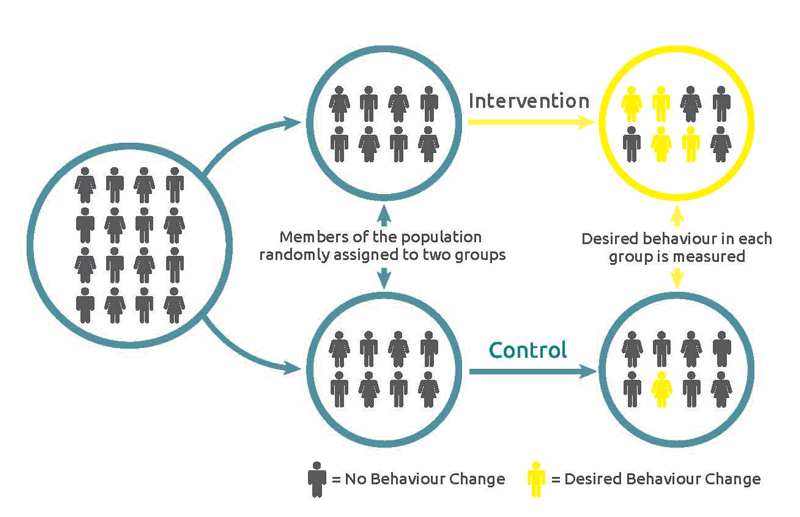
\includegraphics[width = 0.7\textwidth]{fig/RCT.jpg}
        \end{center}


    \begin{itemize}
       
        \item Example: Zhongfei Xingnao Fang \href{https://www.thelancet.com/journals/lancet/article/PIIS0140-6736(24)02261-X/abstract}{(link)}

        
    \end{itemize}
    
    
\end{frame}


\begin{frame}{ATE Under RCT}
    \begin{itemize}

        \item Random assignment implies $$(y_{1i}, y_{0i} ) \bot D_i.$$ The potential outcome is independent of the assignment.

        \bigskip
    
        \item \textbf{Treatment group} ``$\mathcal{T}$'' ($N_1$ observations) 
        \item \textbf{Control group} ``$\mathcal{C}$'' ($N_0 = N - N_1$ observations)
        \begin{align*}
         \widehat{ATE} & = \frac{1}{N_1} \sum_{i \in \mathcal{T}} y_i  - \frac{1}{N_0} \sum_{i \in \mathcal{C}}  y_i \\
             & = \frac{1}{N} \sum_{i=1}^N \left[  \frac{ D_i y_i}{N_1 / N}  -  \frac{(1-D_i) y_i}{N_0 / N} \right]
        \end{align*}
    \end{itemize}
    
\end{frame}


\begin{frame}[plain]{RCT in Development Economics}
    \begin{itemize}
        \item Nobel prize 2019: Banerjee, Duflo, and Kremer
        \begin{itemize}
            \item Deworming in Kenya \href{https://dec.uchicago.edu/insights/1754/}{(link)}
            \item Microcredit in India
        \end{itemize}

        \item  Example in Gansu, China \href{https://www.povertyactionlab.org/fr/evaluation/impact-eyeglasses-academic-performance-primary-school-students-china}{(link)}
        \bigskip
        
        \item Very costly
        \item Few researchers have the resources
    \end{itemize}
\begin{center}
    
\includegraphics[width = 0.6\textwidth]{fig/deworm.jpg}
\end{center}

    
\end{frame}


\begin{frame}[plain]{RCT in Tech Industry}
    \begin{center}
        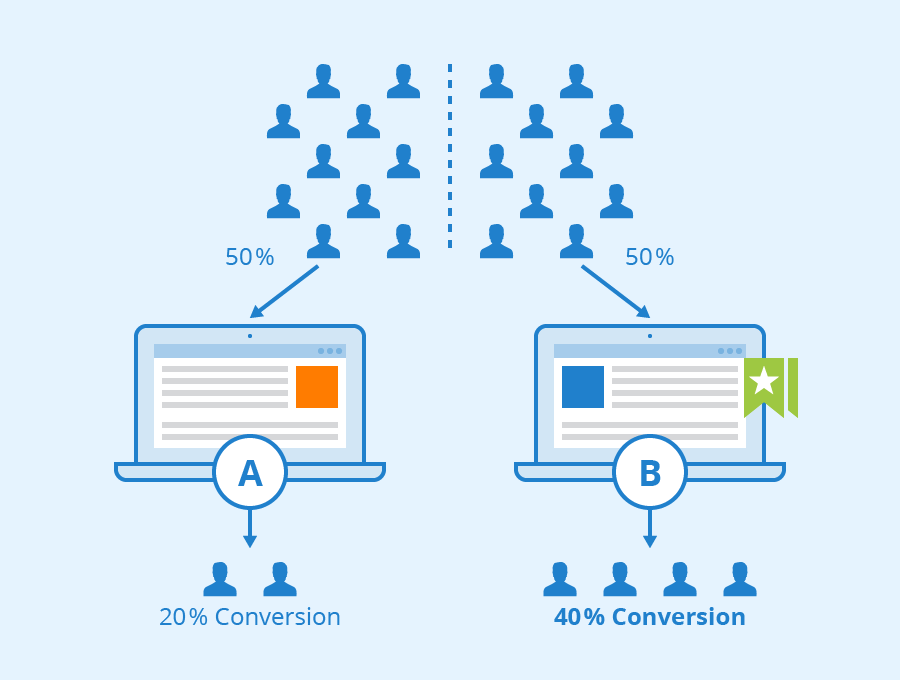
\includegraphics[width = 0.85\textwidth]{fig/AB-Testing.png}
    \end{center}
\end{frame}


\section{Observational Studies}
\frame{\sectionpage}


\begin{frame}{Conditional ATE and ATET}
    \begin{itemize}
        \item With control variables $X_i = x$, \textbf{conditional ATE} (CATE)
        $$ATE(x) = E[ \Delta_i | X_i = x ]$$
        \item Similar, \textbf{conditional ATET} is defined as 
        $$ATE(x) = E[ \Delta_i | D_i = 1 X_i = x ]$$
        \item Straightforward if $X_i$ is a discrete random variable
    \end{itemize}
\end{frame}



\begin{frame}{Unconfoundedness}
    \begin{itemize}
        
        \item To mimic RCT, it requires \textbf{Conditional Independence}
        \[ \left( y_{1i}, y_{0i} \right) \bot D_{i} \mid X_{i} \]
        which is also called \textbf{Unconfoundedness}
        \bigskip 
                \item In an \textbf{observational study}, it means ``Once $X_i$ is controlled, the potential outcome is independent of the treatment''
                
        \item In principle, we should include all \textbf{confounding variables}
        \item Unconfoundedness is an untestable assumption!

        \bigskip
        
        \item $ATET(x) = ATE(x)$ under unconfoundedness.
        \[
        E\left( \Delta_{i} \mid D_{i} =1, X_{i} \right) = E\left( \Delta_{i} \mid X_{i} \right)
        \]  



    \end{itemize}
\end{frame}

\begin{frame}{Overlapping Condition}
    \begin{itemize}
       \item A necessary condition 
       $$ \Pr \left( D_{i} = 1\mid X_{i} = x \right) \in (0,1) $$ 

        \item In the subsample $\{X_i = x\}$, define $\mathcal{T}_x$, $\mathcal{C}_x$, $N_x$, $N_{x,1}$, and $N_{x,0}$  accordingly. Then
        \begin{align*}
            ATE(x) & = E\left( y_{1i} - y_{0i} \mid X_{i} = x \right)  \\
             &  \overset{\text{C.I.}}{=} E\left( y_{1i} - y_{0i} \mid D_{i}, X_{i} = x \right)\\
             \widehat{ATE}(x)  & = \frac{1}{N_{x,1}} \sum_{i \in \mathcal{T}_x} y_i  - \frac{1}{N_{x,0}} \sum_{i \in \mathcal{C}_x}  y_i  \\
             & = \frac{1}{N_x} \sum_{i=1}^N \left[  \frac{ D_i y_i}{N_{x,1} / N_x}  -  \frac{(1-D_i) y_i}{N_{x,0} / N_x} \right]
        \end{align*}
        
    \end{itemize}
\end{frame}


\begin{frame}{Continuous $X$}
    \begin{itemize}
        
        \item The above analysis is based on discrete $X_i$. 
        % \item Assume unconfoundedness and overlapping, and then $$ATE\left(x\right) = ATET \left(x\right)$$ at each point $x$

    \bigskip
        
        \item If $X$ is continuous, one way is to nonparametrically estimate 
        \[m_{j} \left( x \right) = E\left[ y_{ji}  \mid X_{i} = x\right],\, \mbox{for }\, j \in \left\{ 0,1 \right\}\]

        $$ATE(x) = m_1(x) - m_0(x)$$
        
        \item It involves nonparametric estimation techniques that we don't cover

        \item Average $ATE(X_i)$ over the support of $X_i$:
        \[ATE = E\left[ ATE\left(X_i\right) \right] = \int ATE \left(X_i\right) \, \mathrm{d}F\left( X_i \right)\]
        % \item Intuition: $E\left( y_{i} \mathbb{I} \left( D_{i} = 1 \right) \right) = E\left( y_{1i} \right) P \left( D_{i} = 1 \right)$ \\need to adjust for the factor $P\left( D_{i} = 1 \right)$.
        
    \end{itemize}    
\end{frame}

\begin{frame}{Propensity Score}
    \begin{itemize}
        
        \item \textbf{Propensity score}: $$P\left(x \right) = \Pr \left( D_{i} = 1 \mid X_{i} = x \right) = E \left( D_{i}  \mid X_{i} = x \right) $$
        \item In the treatment group
        \begin{align*}
        E\left( \frac{D_{i} y_{i}}{P\left( X_{i} \right)} \right) 
         & \overset{\text{LIE}}{=}  E\left( \frac{1}{P\left( X_{i} \right)} E\left( D_{i} y_{1i} \mid X_{i}\right) \right) \\
         & \overset{\text{C.I.}}{=} E \left( \frac{1}{P\left( X_{i} \right)} E \left( D_{i} \mid X_{i} \right) E\left(y_{1i} \mid X_{i} \right)\right) \\
         & = E \left(  E\left(y_{1i} \mid X_{i} \right)\right) 
         \overset{\text{LIE}}{ = } E\left( y_{1i} \right)    
        \end{align*}
        
    \end{itemize}
\end{frame}



\begin{frame}{ATE Under Continuous $X$}
    \begin{itemize}

        \item Similarly,  in the control group $E\left( \frac{\left( 1 - D_{i} \right)y_{i}}{1 - P \left( X_{i} \right)} \right) = E\left( y_{0i} \right)$
        
    
        \item The (unconditional) ATE is 
        $$ ATE = E\left( \frac{D_{i}y_{i}}{P \left( X_{i} \right)} - \frac{\left( 1 - D_{i} \right) y_{i}}{1 - P\left( X_{i} \right)} \right) $$
        \begin{itemize}
            \item Important to ensure $P(X_i) \in (0,1)$. Logistic.
        \end{itemize}
        
    \end{itemize}
\end{frame}








\begin{frame}{Linear Regression}
    \begin{itemize}
        \item Linear regression
        \begin{align*}
        y_i & = \alpha + X'_{i} \beta + \varepsilon_{i}
        \end{align*}
        under the assumption $E [ \varepsilon_i | X_i ] = 0$ implies that if $X_i$ is a scalar (the simplest case), then
        $$ \beta = \frac{E[y_i | X_i = x_1 ] - E[y_i | X_i = x_0 ]}{ x_1 - x_0}$$ for any $x_0,x_1 \in \mathcal{X}$. 
        \item The slop coefficient is the difference between two groups. 
    \end{itemize}
\end{frame}





\begin{frame}{Interpretation of Linear Regression: I}
    \begin{itemize}
        \item Linear regression is a purely statistical exercise, just like the comparison of two means.
        \item Example: Wage gap in gender
        
\bigskip

        \item $E[y_i | X_i]$ always exists, but the linear regression may not get the ``causal'' effect

        
        
        
    \end{itemize}
\end{frame}

\begin{frame}{Example: Omitted Variable Bias}
    \begin{itemize}
        \item The causal model
            \[y_i = \alpha + \beta X_i + \gamma Z_i + \varepsilon_i, \quad \text{with}\, E\left[\varepsilon_i \mid X_i, Z_i \right] = 0\]
            but $Z_i$ is omitted from regression
        \item Linear regression of $y_i$ on $X_i$ can still be implemented:
            \[E\left[ y_i\mid X_i\right] = \alpha + \beta X_i + \gamma E\left[Z_i\mid X_i \right] = \alpha + \theta X_i\]
            where $$\theta = \beta + \gamma \frac{\mathrm{Cov}\left( X_i, Z_i \right)}{\mathrm{Var}\left( X_i \right)}$$
    \end{itemize}
\end{frame}




\begin{frame}{Omitted Variable Bias (Cont.)}

        
       %  Example: $y$ is salary, $X$ is college entrance.
        
        \begin{itemize}
           %  \item Linear regression is not``causal''. When worried about endogeneity, we have a causal model in mind.


        \item The reduced form $$y_i = \alpha + \theta X_i + u_i$$ ensures $E\left[ u_i \mid X_i \right] = 0$ (under joint normality), but this is not a causal model.  
        \item From the observational data, we cannot shift  $X_i$ without shifting $u_i$ simultaneously.


           % \begin{align*}
           % y_i & = \alpha_1 + \beta D_i + \varepsilon_i     \\
           % E[y_i|D_i]  & = \alpha_1 + \beta D_i + E[\varepsilon_i |D_i] \\
           % E[y_i|D_i=1] - E[y_i|D_i=0]  & = \beta D_i \\ 
           %  & +  (E[\varepsilon_i |D_i=1] -  E[\varepsilon_i |D_i=0]) 
           % \end{align*}

            
            
            \item Causal question cannot be answered without further structures.

        \bigskip
        
            \item Importance of the causal model: Only the causal relationship has policy implications.
        \end{itemize}

\end{frame}





\begin{frame}{Regression-based Causal Model}
    \begin{itemize}

        \item Continue with the example: Change the year of education. 
        
        \item ``Keeping everything else equal, if a person's $X_i$ is changed from $x_0$ to $x_1$, then $\beta$ is the average change of $y_i$.'' This is a potential outcome claim.
    
        \item Given $D_i\in \{0,1\}$ there are two potential outcomes
        \begin{align*}
        y_{0i} & = \alpha_{0} + X'_{i}\beta_{0} + \varepsilon_{0i}\\
        y_{1i} & = \alpha_{1} + X'_{i}\beta_{1} + \varepsilon_{1i}
        \end{align*}
        The linear assumption makes life easier under continuous $X_i$.

    \end{itemize}
\end{frame}



\begin{frame}{CATE}
    \begin{itemize}

        
        \item The above model implies \textbf{heterogeneous treatment effect}
        \[\Delta_{i} = \left( \alpha_{1} - \alpha_{0} \right) + X'_{i} \left( \beta_{1} - \beta_{0} \right) + \left( \varepsilon_{1i} - \varepsilon_{0i}\right)\]
        \item By construction $E\left( \varepsilon_{1i} \mid X_{i} \right) =  E\left( \varepsilon_{0i} \mid X_{i} \right) = 0$, and thus
        
        \[ATE(X_i) =  E\left( \Delta_{i} \mid X_{i} \right) =  \left( \alpha_{1} - \alpha_{0} \right) + X'_{i} \left( \beta_{1} - \beta_{0} \right)\]

        \item If $\beta_1 = \beta_0$, then $ATE(X_i) = \alpha_{1} - \alpha_{0} $ is a level change homogeneous to all people
        
    \end{itemize}
\end{frame}



\begin{frame}{Selection Bias}
\begin{align*}
   ATET(X_i) & = E\left( \Delta_{i} \mid D_{i} =1, X_{i} \right) \\
    & = ATE(X_i) + E\left( \varepsilon_{1i} - \varepsilon_{0i} \mid D_{i} =1, X_{i} \right) 
\end{align*}

    \begin{itemize}
         
        \item Under unconfoundedness, $ATE(X_i) = ATET(X_i)$
        \item Otherwise, \textbf{selection bias} if $$E\left( \varepsilon_{1i} - \varepsilon_{0i} \mid D_{i} =1, X_{i}  \right) \ne 0$$
        The individual knows $\varepsilon_{1i} - \varepsilon_{0i}$, and he elects to the treatment group because of that.
        
    \end{itemize}
\end{frame}




\begin{frame}{Self-Selection}

    \begin{itemize}

         % \item The fact that a person joins the treatment group is a calculated rational decision, not an indifferent random assignment.
        \item Example: College premium
        \begin{itemize}
            \item Treatment: college entrance $D_i$
            \item The unconfoundedness $$(\varepsilon_{i,0}, \varepsilon_{i,1}) \bot D_i \, | \, \text{X}_i$$ does not hold in general. \bigskip
        \end{itemize}

        \item The linear regression does not provide credible causal interpretation.
        \item Need other techniques to estimate causality.
        
    \end{itemize}
\end{frame}



% I would like to talk about LATE.
% However, LATE is not covered by the textbook

\section{Quasi experiment}
\frame{\sectionpage}

\begin{frame}{Regression Discontinuity Design}
    \begin{itemize}
        \item A jump point due to some ad hoc policy cutoff
        \item Unconfoundedness is naturally satisfied
        \item e.g.~The value-added of college
        \item Caveat: valid only for the subpopulation around the cutoff
        \item Suppose the cutoff is $c$
        \item $y_{0i} = \alpha_0 + \beta_0 (x_i - c) + \varepsilon_{0i}$
        \item $y_{1i} = \alpha_1 + \beta_1 (x_i - c) + \varepsilon_{1i}$        
    \end{itemize}
\end{frame}




\begin{frame}{Example: Air Pollution in Huai River}
\begin{itemize}
    \item Chen, Ebenstein, Greenstone, and Li (2013, PNAS) 
\end{itemize}

\begin{figure}
    \centering
    \begin{subfigure}{0.45\textwidth}
        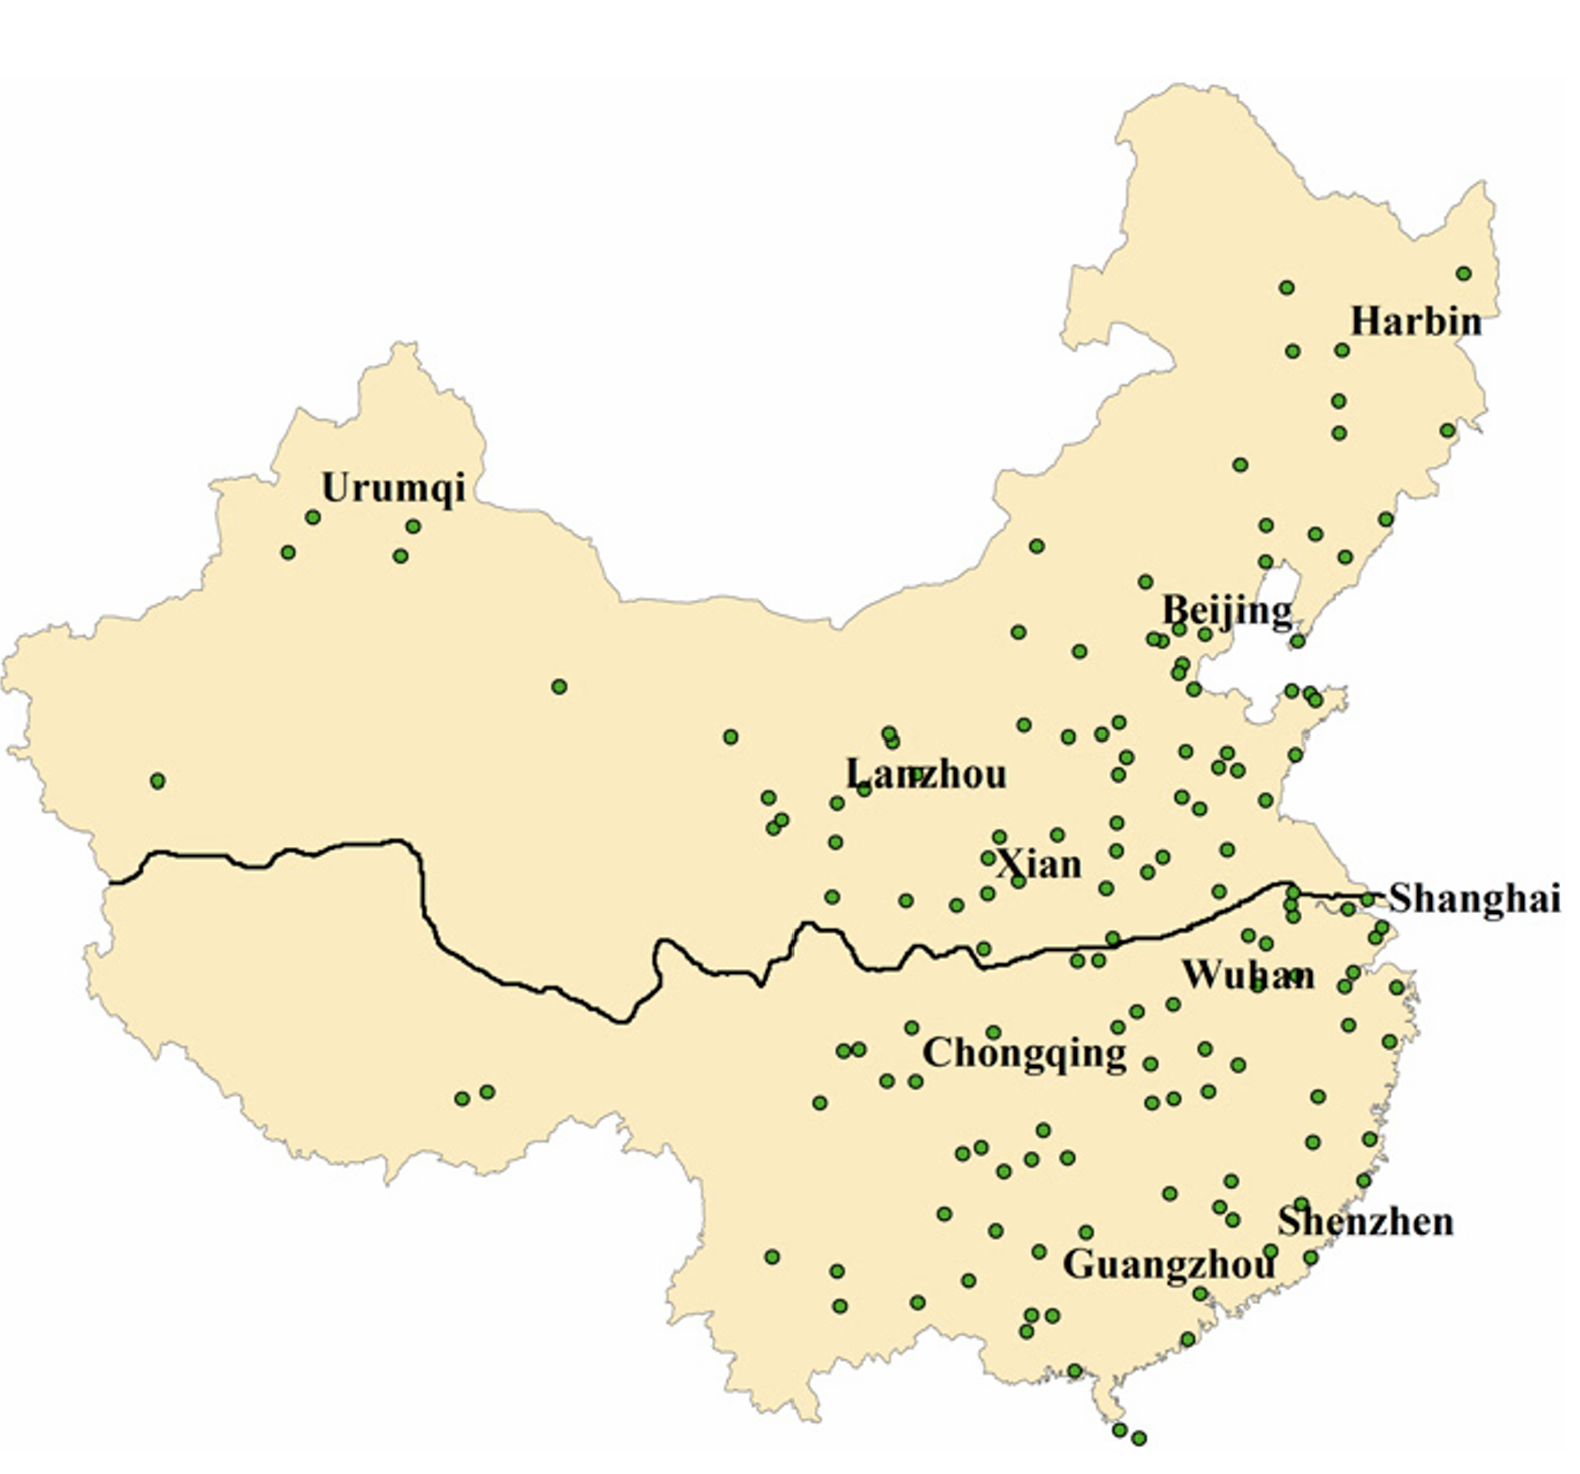
\includegraphics[width=\textwidth]{fig/Huai_river.png}
    \end{subfigure}
    \hfill
    \begin{subfigure}{0.45\textwidth}
        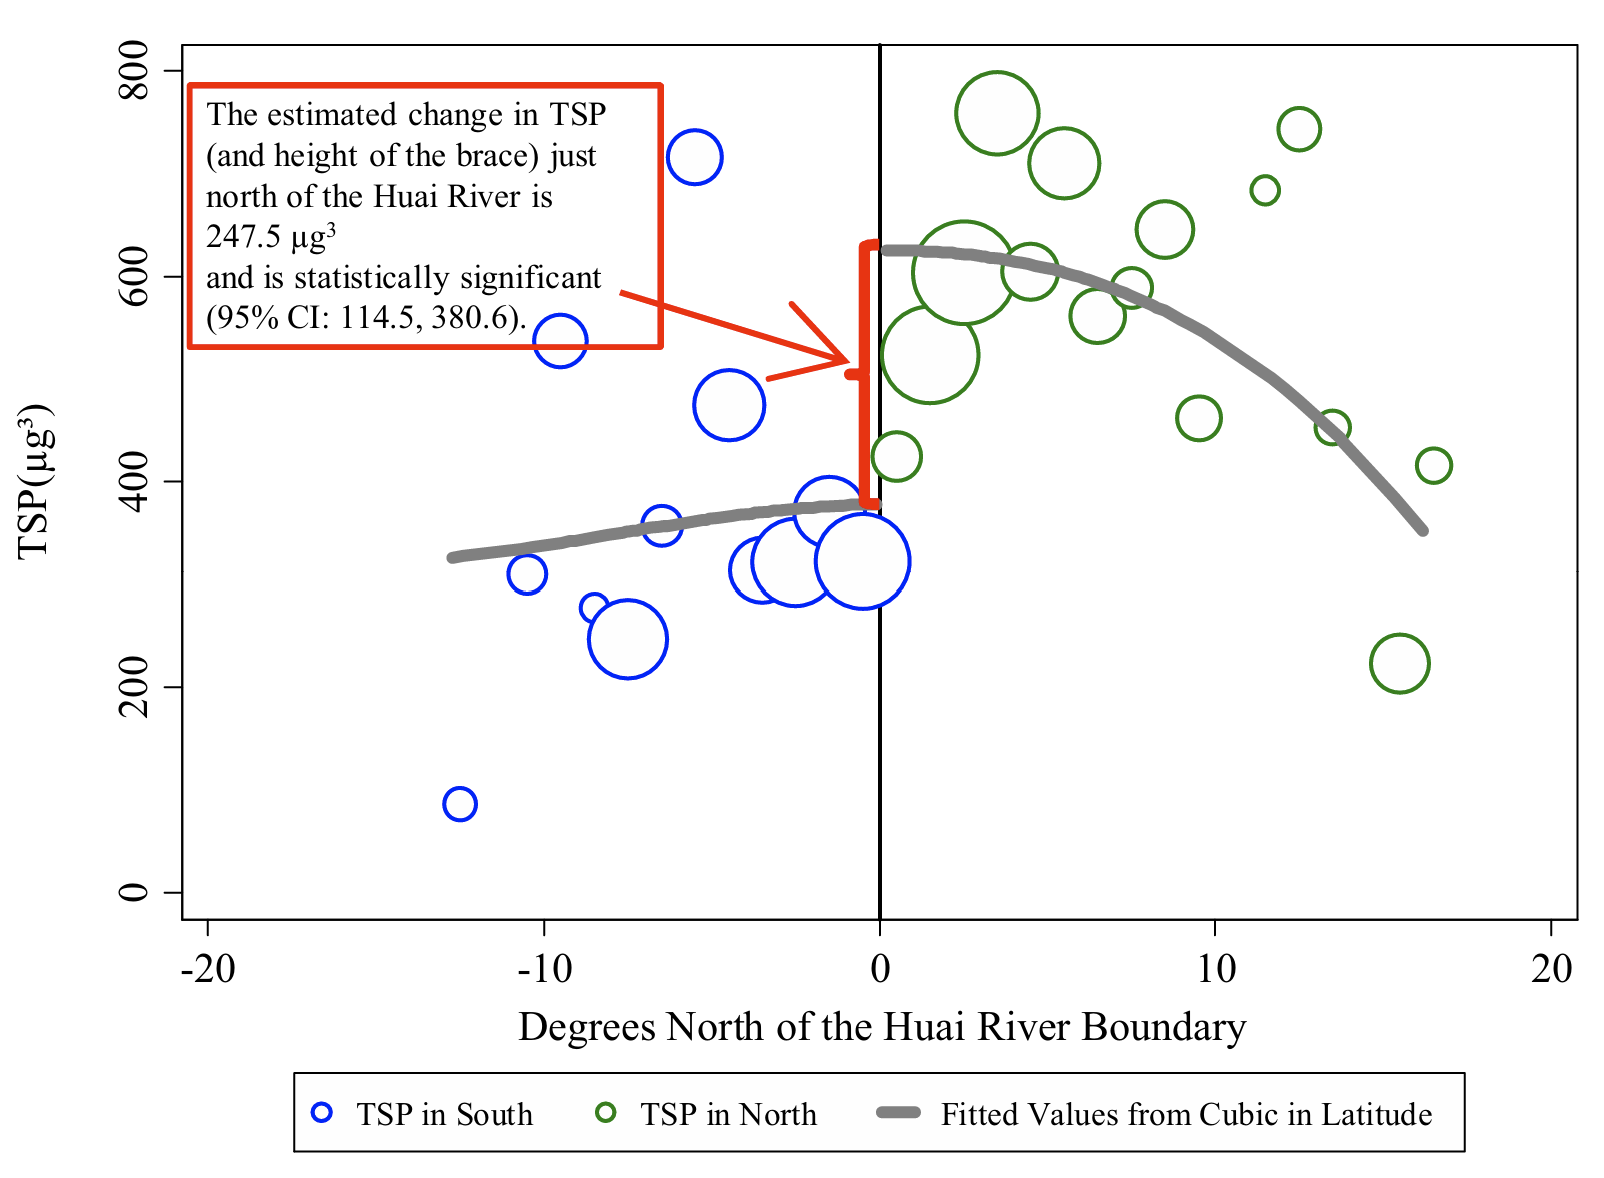
\includegraphics[width=\textwidth]{fig/RDD_Huai.png}
    \end{subfigure}
\end{figure}
    
\end{frame}

    



\begin{frame}{Event Study}
\begin{itemize}
    \item A time series topic, but very similar to treatment
    \item The same individual observed over time $t = 1,2,\ldots,T$
    \item An event happens at time $t = T_1$
    \begin{itemize}
        \item Before event (control group);  After event (treatment group)
        
    \end{itemize}

    \begin{center}
        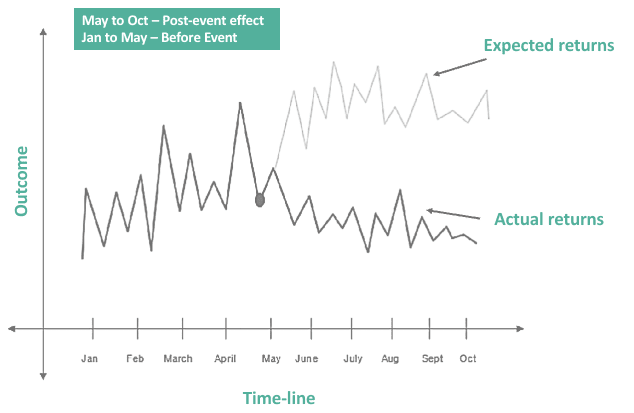
\includegraphics[width = 0.6 \textwidth]{fig/Event-Study.png}
    \end{center}
    
\end{itemize}
\end{frame}
 

\begin{frame}{Implementing Event Study}
\begin{itemize}
    \item Let $D_t = \mathbb{I}(t \geq T_1) $
    \item Regression
    $$y_t = \alpha + \beta D_t+ \varepsilon_t$$
    \item Key assumption
    $$E[\varepsilon_t | D_t ] = 0 \mbox{ for all } t = 1,2\ldots,T $$
    \item Other control variables can be added into the regression

\bigskip

    \item My 2004 undergraduate thesis
    
\end{itemize}
\end{frame}




\begin{frame}{Difference-in-Difference (DID)}
    \begin{itemize}

        \item Two groups, two periods (simple panel data)
        \begin{itemize}
            \item The two groups are naturally different
            \item \textbf{Parallel trend} over time. This is an assumption!
        \end{itemize}
        
        \item One of the most popular empirical techniques

        \bigskip

        \item Example: North Korea and South Korea
    \end{itemize}



    
\end{frame}



\begin{frame}{Implementing DID}

\begin{itemize}
    \item Two indicators $D_i$ and $D_t$
    \item Regression is convenient for hypothesis testing
    $$y_{it} = \beta_0 + \beta_1 D_i + \beta_2 D_t + \beta_3 \cdot D_i D_t + \epsilon_{it}$$
    \item Other control variables can be added
\end{itemize}


\begin{center}
    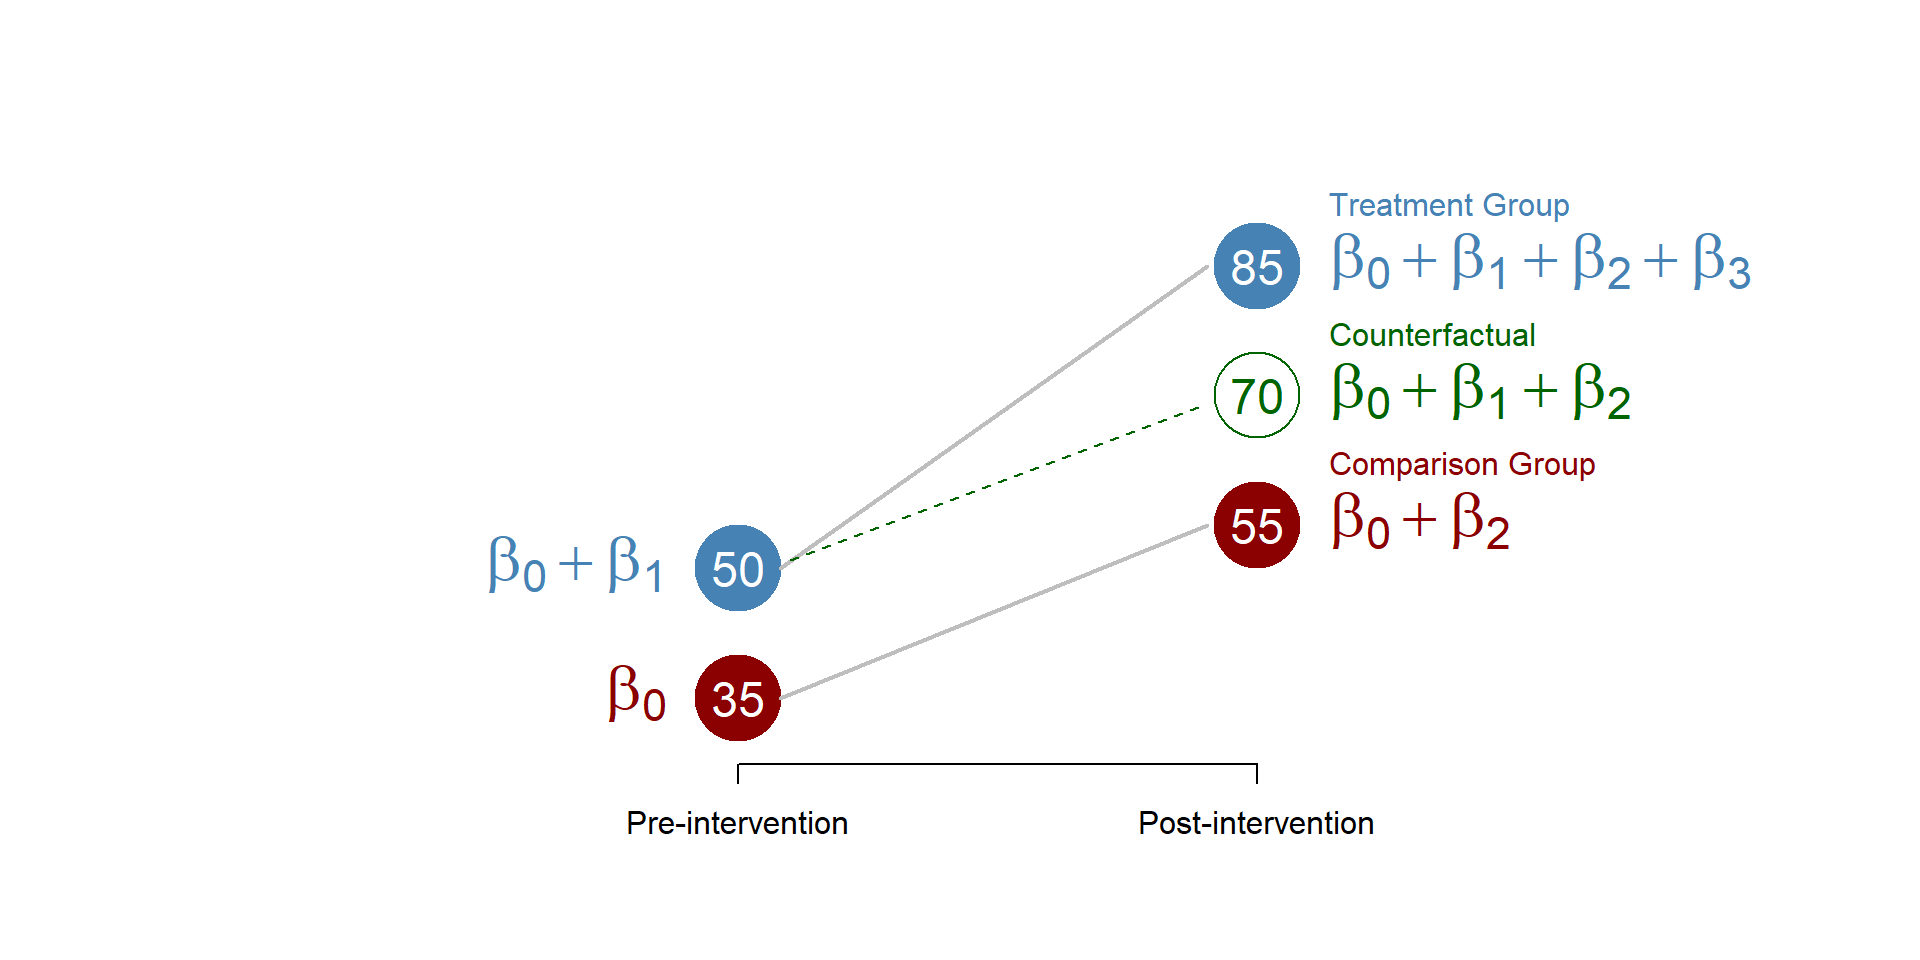
\includegraphics[width = \textwidth]{fig/diffindiff.png}
\end{center}
    
\end{frame}

\begin{frame}{Summary}
\begin{itemize}
    \item Potential outcome framework
    \item RCT
    \item Propensity score
    \item Regressions for CATE
    \item RDD
    \item DID

    \bigskip
    \item Popular in academia as well as tech sector
        \href{https://arxiv.org/abs/2007.05188}{(link1)},
        \href{https://www.bilibili.com/video/BV1VW4y1y7AR/?spm_id_from=333.337.search-card.all.click&vd_source=a4b181aa9857818286999eec4d9925e6}{(link2)}
        
    \begin{itemize}
        
        \item \href{https://www.zhipin.com/job_detail/e7fa10b466e0c5e41HV82ty9EFdW.html?lid=51us4b3FXFX.search.6&securityId=wnbs_9BkN5Fhf-l1orLT94YWn2kpcjBS6-5X6P4y3qOfoxGDb-LqdsKmwiPycwn1pnZbvF3A-M69do0VjdtCM5SeBd6a_1lLChm-XpGGAe7ZWlB7Hw~~&sessionId=}{Bytedance}

        \item \href{https://www.zhipin.com/job_detail/750563b6c1b42dc11HJ_29y6FVJX.html?lid=51ns09pI55u.search.1&securityId=gnIJonr0XicLr-u1wfIDvyBCsowYfmBnKb7KPziKxfWxaujP30mDd7MWcogl4qQIsW0il0VtOVllz_u0bVWfEswvyt94fI3NKEObdTFdhBDTXwA~&sessionId=}{Kuaishou}

        \bigskip 

        
    \end{itemize} 
\end{itemize}
\end{frame}

\begin{frame}[plain]{Related Work of Mine}

    \begin{itemize}
        \item  Zhentao Shi and Jingyi Huang (2023): “Forward-Selected Panel Data Approach for Program Evaluation,” Journal of Econometrics, 234(2), 512-535.
    \end{itemize}

    \begin{center}
        
\includegraphics[width = 0.63\textwidth]{fig/amazon.PNG}
    \end{center}
    
\end{frame}




\end{document}